\documentclass{beamer}
\usetheme[pageofpages=of,% String used between the current page and the
                         % total page count.
          bullet=circle,% Use circles instead of squares for bullets.
          titleline=true,% Show a line below the frame title.
          alternativetitlepage=true,% Use the fancy title page.
       %   titlepagelogo=logo-polito,% Logo for the first page.
       %   watermark=watermark-polito,% Watermark used in every page.
       %   watermarkheight=100px,% Height of the watermark.
       %   watermarkheightmult=4,% The watermark image is 4 times bigger
                                % than watermarkheight.
          ]{Torino}

\setbeamertemplate{footline}{
  \begin{beamercolorbox}[wd=\paperwidth,ht=1ex,dp=1ex]{footline}
    \vspace{5pt} \hspace{1em} \insertframenumber/\inserttotalframenumber
  \end{beamercolorbox}
}

\author{Brendon J. Brewer}
\title{STATS 331 -- Introduction to Bayesian Statistics}
\institute{The University of Auckland}
\date{}


\linespread{1.3}
\usepackage{minted}
\usepackage[utf8]{inputenc}
\usepackage{dsfont}
\newcommand{\given}{\,|\,}


\begin{document}

\frame{\titlepage}

\begin{frame}
\begin{center}
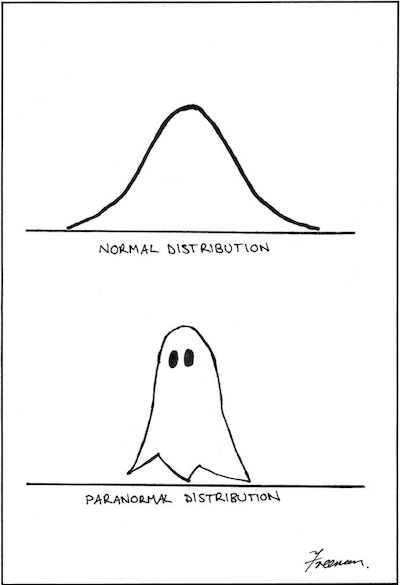
\includegraphics[width=0.4\textwidth]{images/paranormal.png}

Credit: Matthew Freeman
\end{center}

\end{frame}



\begin{frame}
\centering
\large
Heavy-Tailed Models and Multiple Regression

\end{frame}


\begin{frame}
\frametitle{Fake Data with Outlier}
I generated some data from $y=x$ with $\sigma=1$, then manually added two
extreme outliers:

\begin{center}
\includegraphics[width=0.6\textwidth]{images/outlier_data.pdf}
\end{center}

\end{frame}

\begin{frame}
\frametitle{Fake Data with Outlier}
\begin{itemize}
\item What will happen if we run the linear regression model, as it is, on this
data? \pause
\item The classical least squares estimate would be dragged substantially towards
the outliers (by reducing the slope).\pause
\item With the current model, the same thing will happen in the Bayesian framework,
because of the choice of sampling distribution/likelihood --- particularly,
the light tails of the gaussian.
\end{itemize}
\end{frame}

\begin{frame}
\frametitle{Running the Model}
Let's run the regression model on this data, and see what the posterior
distributions look like, and whether they accurately recover
$y=x$ and $\sigma=1$.\pause

Surprisingly, the posterior distributions for $\beta_0$ and $\beta_1$ aren't
actually that bad, but the uncertainties get inflated because $\sigma$ has
to be super high to explain the outliers.
\end{frame}


\begin{frame}
\frametitle{Conclusion}
The best way of explaining this data, with the current model, is if $\sigma$
is much larger than 1 and the slope $\beta_1$ is less than 1.
{\bf If we believe the model assumptions}, this is the
answer, and that's that.\pause

However, often model assumptions aren't truly reliable but are chosen out of
tradition or habit. We are free to change the model to one that
{\bf expects} the odd outlier.
\end{frame}


\begin{frame}
\frametitle{Student-$t$ Distributions from Wikipedia}

\begin{center}
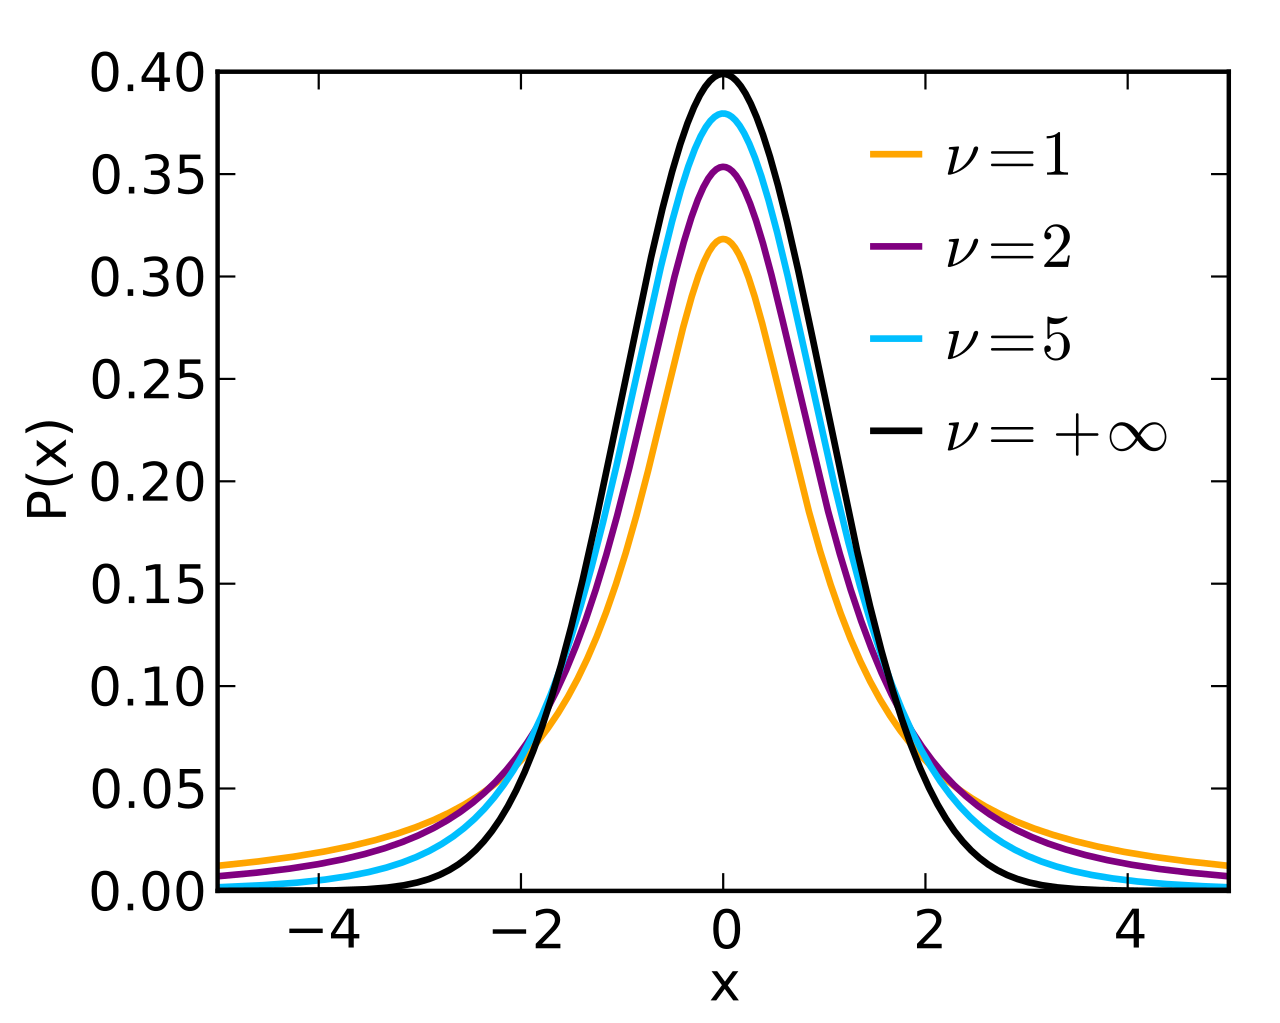
\includegraphics[width=0.7\textwidth]{images/t_distribution.png}
\end{center}
\end{frame}

\begin{frame}[fragile]
\frametitle{Student-$t$ Distributions in JAGS}
We will use the Student-$t$ distribution as a drop-in replacement for the
normal distribution in our model. We simply replace
\begin{minted}{r}
dnorm(mu, 1/sigma^2)
\end{minted}
with
\begin{minted}{r}
dt(mu, 1/sigma^2, nu)
\end{minted}
\pause
{\bf Note}: The extra parameter \mintinline{r}{nu}, which controls the
tail behaviour, will need a prior (low $\nu$ = heavy tails,
high $\nu$ = approximately normal).
\end{frame}

\begin{frame}[fragile]
\frametitle{Modified Parts of the Regression Model}
\footnotesize
\begin{minted}{r}
log_nu ~ dunif(-2, 5)
nu <- exp(log_nu)

for(i in 1:length(y))
{
    y[i] ~ dt(beta0 + beta1*(x[i] - mean(x)), 1/sigma^2, nu)
}
\end{minted}
\pause

{\bf Note}: \mintinline{r}{sigma} is no longer a standard deviation, but is still
a scale parameter (controls width).

\end{frame}


\begin{frame}[fragile]
\frametitle{Results from Heavy-Tailed Model}
The results from the heavy tailed model are a fair bit better,
and $\sigma$ (even though it has changed its interpretation a bit)
is much smaller. It can explain the outliers by having a low value
of $\nu$ instead.\\[0.5em]\pause

We can look at the posterior for $\log(\nu)$ (which had a uniform prior)
to see, whether large values (i.e., approximately gaussian shape) are ruled out.

\end{frame}

\begin{frame}[fragile]
\frametitle{One Parameter Space}
Instead of doing model selection (which we cannot do here as MCMC does not
calculate marginal likelihoods), we can sometimes create something like
the two models in the one parameter space, and just do parameter estimation.
This is a good strategy in general.

\end{frame}




\end{document}

